\RequirePackage[l2tabu, orthodox]{nag}
\documentclass[12pt]{article}

\usepackage{amssymb,amsmath,verbatim,graphicx,microtype,upquote,units,booktabs,hyperref,tikz,wrapfig,xcolor,pgfplots,listings,xcolor}
\usepackage[binary-units=true]{siunitx}
\usepackage[margin=10pt, font=small, labelfont=bf, labelsep=endash]{caption}
\usepackage[os=mac, mackeys=symbols]{menukeys}

\pgfplotsset{compat=1.12}
\setcounter{secnumdepth}{2}

\title{Project \#3}
\date{Due Date: Tuesday, December 6\textsuperscript{th}, 2016}
\author{Michael Schoen, Abdirahman Osman, Illya Starikov}

\newcommand{\shellcmd}[1]{\texttt{\colorbox{gray!30}{#1}}}
\newcommand{\todo}[1]{\textbf{\colorbox{red!50}{#1}}}
\newcommand{\br}{\\\multicolumn{2}{c}{} \\ }

\begin{document}
\maketitle

For the second project, we were delighted to be able to use a higher level programming language; we\footnote{Illya.} decided to apply this new-found excitement to implement a retro game from the \num{70}s: Space Invaders.

\begin{figure}[!ht]
    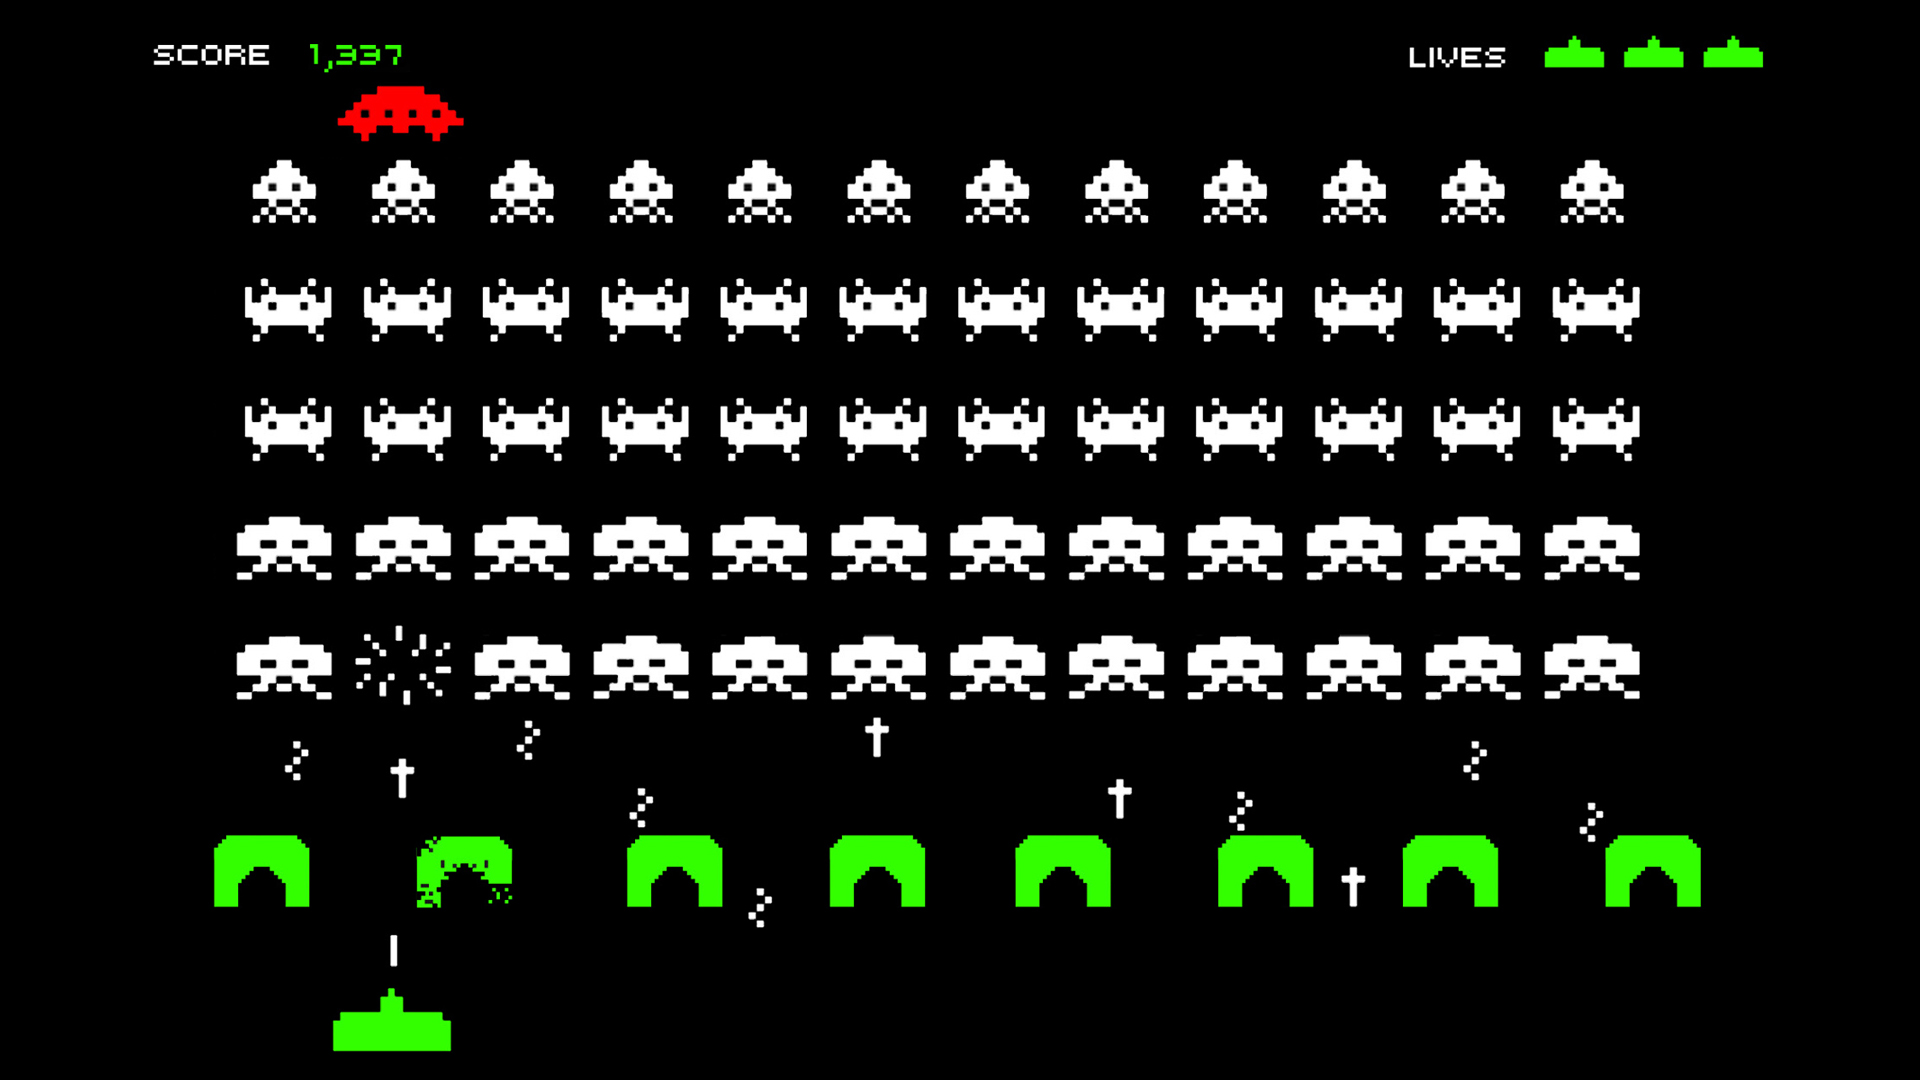
\includegraphics[width=\textwidth]{assets/space-invaders.jpg}
    \caption{The original space invaders.}
    \label{space-invaders}
\end{figure}

\section{Project Description}
Below we will go into more detail about each individual parts of our project.

\subsection{The Game}
The game we initially decided to go with was space invaders. We had intention of doing the game logic on the microcontroller through serial communication; however, we learned early that this was likely not be possible\footnote{Our hex file with very basic functionality was \SI{25}{\kilo\byte}.}. We describe in \textit{Problems Encountered} how we absolved this. From here, we decided our game would exclusively be in the terminal.

Our game essentially creates a two dimensional array (in three segments --- the header to show score and level, the aliens, and the shooter). Then we loop through depending on the input:

\begin{description}
    \item[\keys{\arrowkeyleft}] Move the shooter left.
    \item[\keys{\arrowkeyright}] Move the shooter left.
    \item[\keys{q}] Quits the game
    \item[\keys{\SPACE}] Shoots with the gunner.
    \item[\keys{ }] No input meant refresh game.
\end{description}

We achieved the drawing through curses\footnote{Can be read about here \url{https://en.wikipedia.org/wiki/Curses_(programming_library)}}. Ultimately, we did not get our game fully done, but a good majority of it.

\begin{figure}[!ht]
    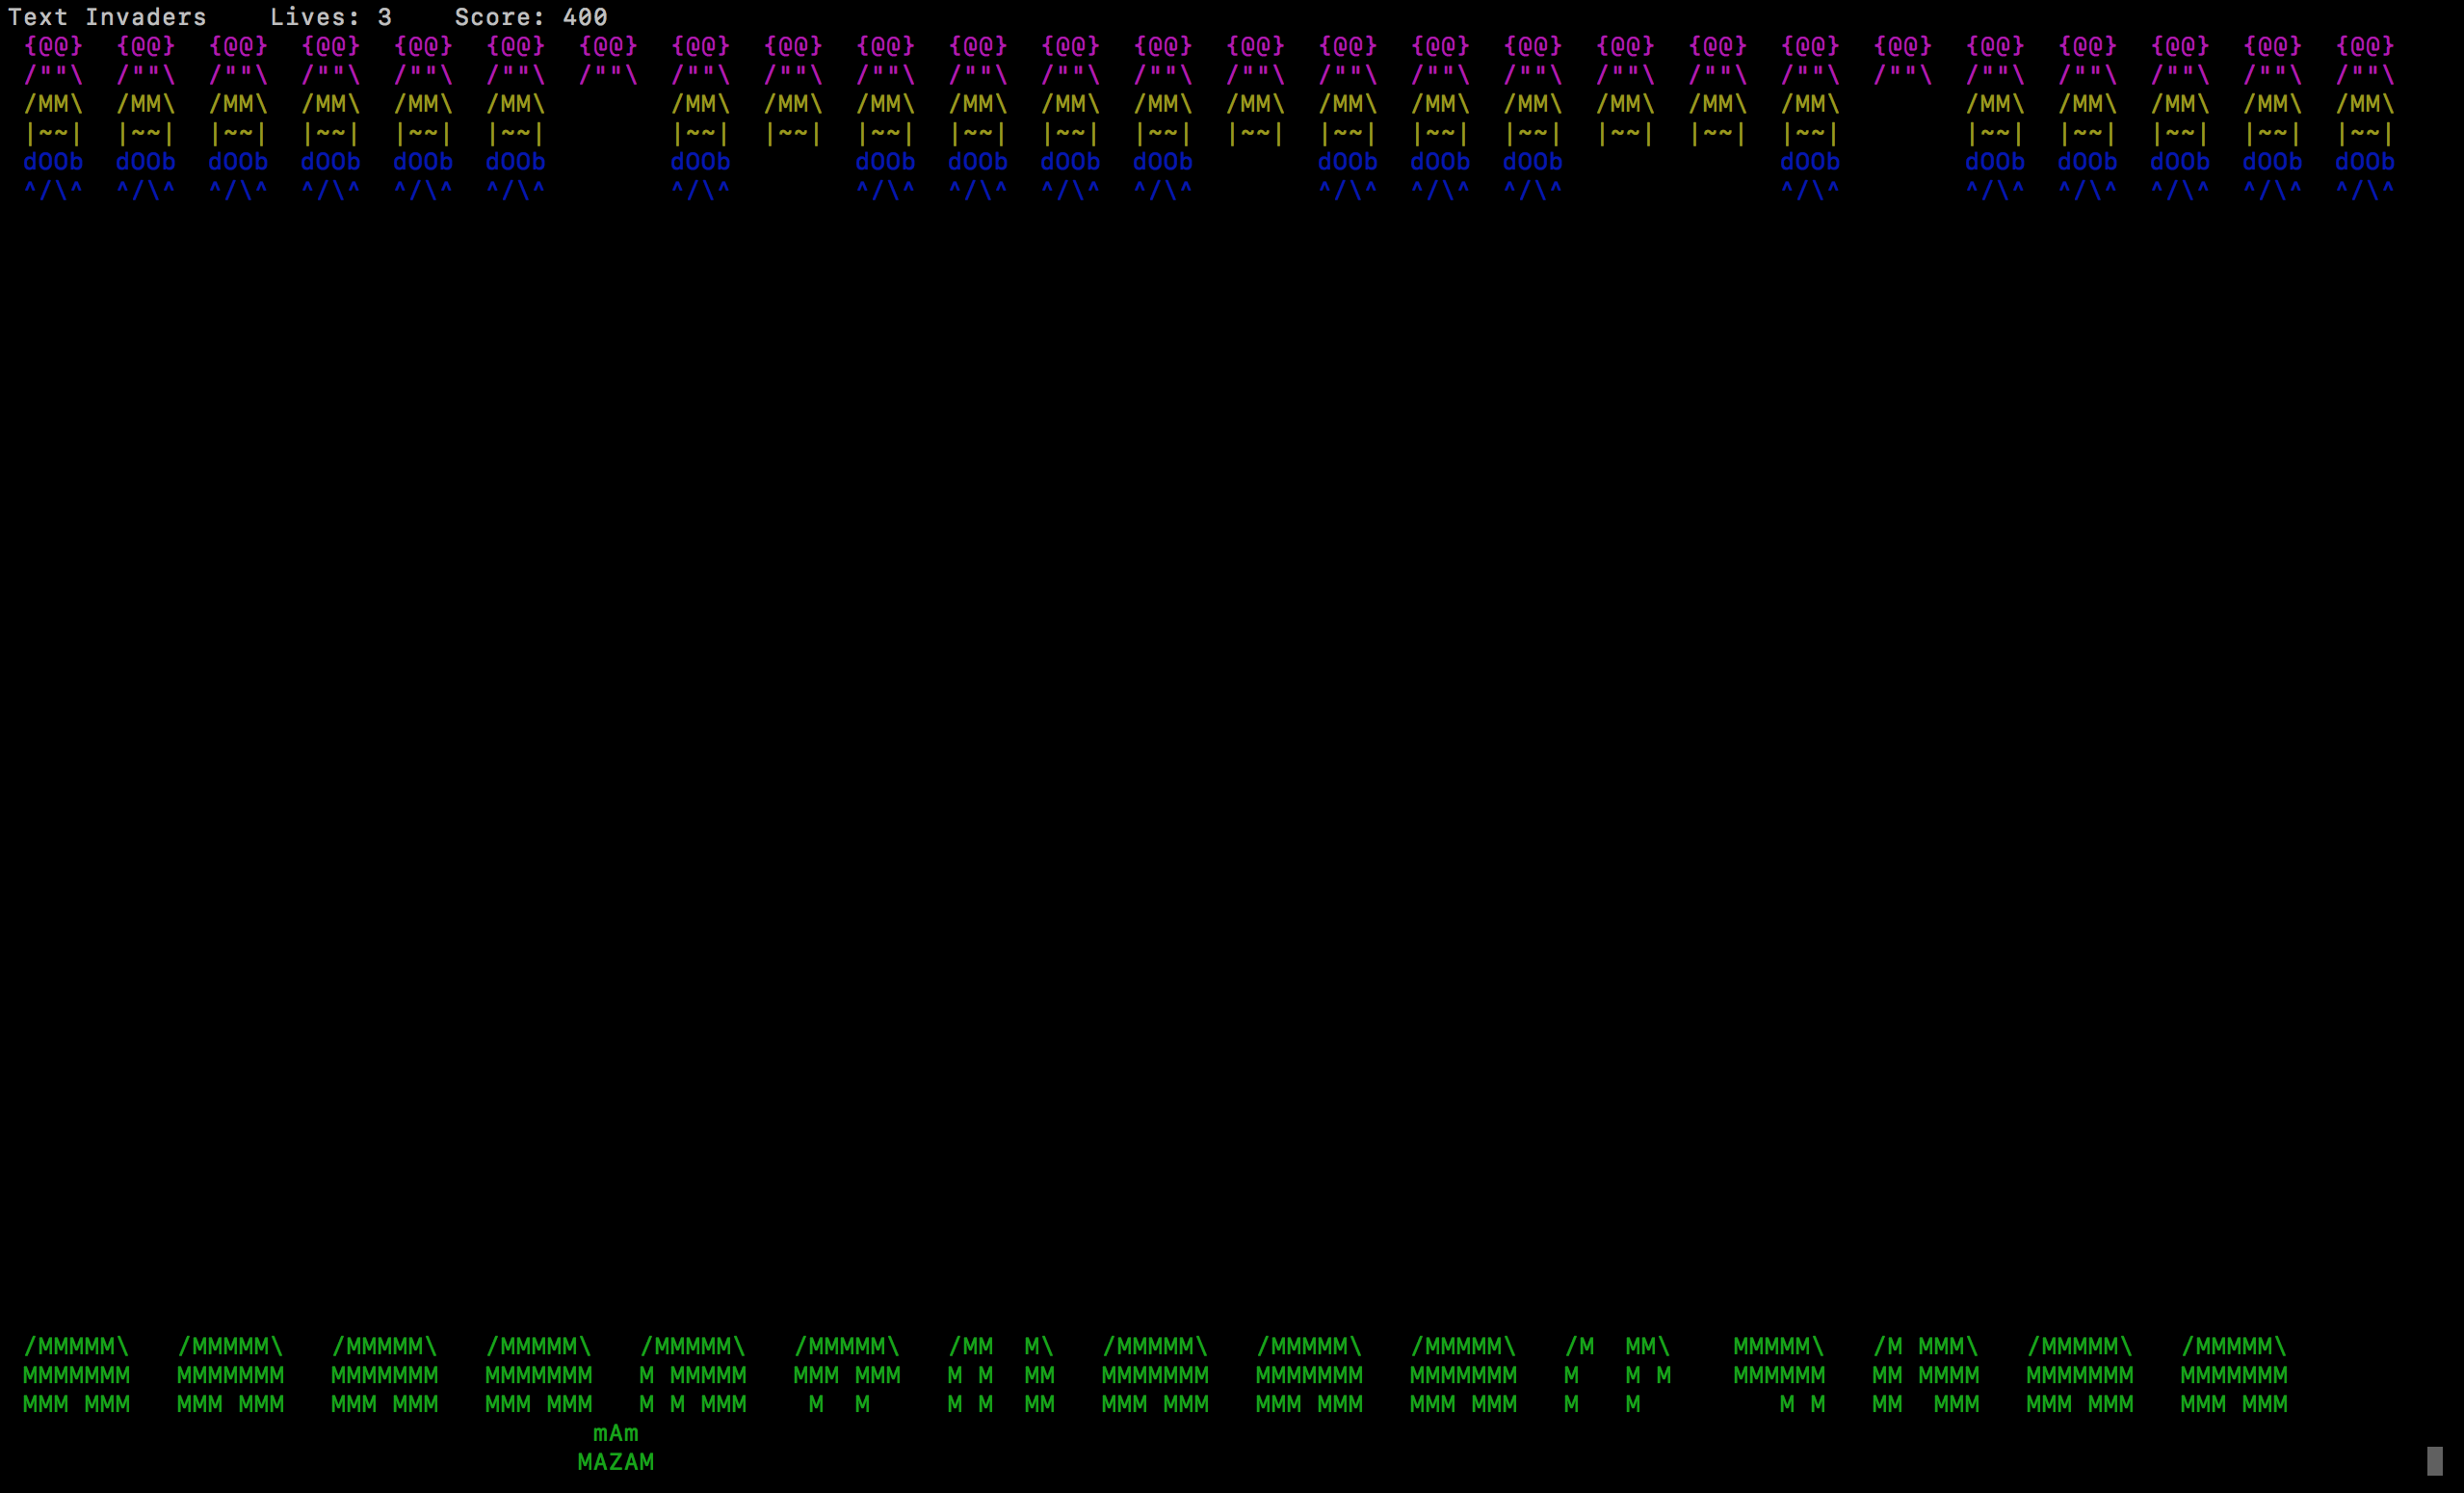
\includegraphics[width=\textwidth]{assets/game.png}
    \caption{Text Invaders, our version of space invaders..}
    \label{game}
\end{figure}

\subsection{Music}
The formula for each note is $$\frac{\nicefrac{1}{4} \, \text{Oscillator Frequency}}{\text{Note Frequency}}$$. To produce the music, we had a function that took in which note and the type of note (\num{16}\textsuperscript{th}, \num{8}\textsuperscript{th}, \num{4}\textsuperscript{th}, half or whole note). The function multiplied the base length of a note by a constant depending on the type of note. A \num{16}\textsuperscript{th} note would be multiplied by \num{1}, an \num{8}\textsuperscript{th} by \num{2}, a quarter note by \num{4}, a half-note by \num{8}, and a whole note by \num{16}. We used timers and interrupts for the period of the note and the length of the note.

We used sheet music to get the notes. For speeding and slowing down the music, the type of note was just multiplied by \num{2} or divided by \num{2} respectively.

\subsection{Seven Segment Display}
For the seven segment display, we had to set $P_2$ to be push/pull so that the display would receive enough power. We then looked up the correct values to output to the pins to make each number show up on the display and used those values in the increment/decremented function as well as the simple function that lets you display any number. We used the data sheet for the seven segment display to see how to connect it on the breadboard.


\section{Problems Encountered}
Below we will list some of the ``several'' problems we ran into.

\subsection{Memory Constraints}
By far, the biggest problem we encountered was the memory constraint. The \SI{8051} has \SI{8}{\kilo\byte} of memory; our code base, with the exclusion of all the \shellcmd{malloc}s\footnote{Since \shellcmd{unsigned char} = \SI{1}{\byte}, the terminal window will roughly be $20\text{ height} \times 80\text{ width} $, we can roughly expect \SI{1.6}{\kilo\byte} to be allocated on the heap; a non-insignificant amount compared to \SI{8}{\kilo\byte}.}, it is roughly \SI{25}{\kilo\byte} --- a size a bit larger than the \num{8051} allows. Our workaround was to fight fire with fire.

Instead of ``dumbing'' down our game\footnote{According to back of the hand calculations, a space-optimized version of the game would still be \SI{7}{\kilo\byte}. This was likely to be impossible.} to get it to fit, we decided to have an external interface; specifically, a port sniffer. It would listen for input from the \num{8051}, and if there is a signal on the serial port, use that as input. If not, default to the keyboard input.

Ultimately, we were unsuccessful with the port sniffer. Originally, we had tried to use a Linux port sniffer so we can just embed it into our program, \shellcmd{slsnif}\footnote{Can be found at \url{https://sourceforge.net/projects/slsnif/}.}. Unfortunately this port sniffer does not support ``legacy'' ports, and the \num{8051} falls in this category. So we moved onto a Windows port sniffer, \shellcmd{Serial Input For Windows}\footnote{Can be found at \url{http://www.randomnoun.com/wp/2013/02/03/serial-input-for-windows/}.}. This too did not work, because we could only have one interface use the serial port, so we would need a dedicated socket to intercept the \shellcmd{COM1} port's input --- something we were not familiar with.

Ultimatly, we were


\section{Individual Features}
\begin{itemize}
    \item Michael Schoen --- 33\% Contribution
    \begin{itemize}
        \item Song
        \item Seven Segment Display
    \end{itemize}

    \item Abdirahman Osman --- 33\% Contribution
    \begin{itemize}
        \item Port Serialization
        \item Menu Logic
    \end{itemize}

    \item Illya Starikov --- 33\% Contribution
    \begin{itemize}
        \item Space Invaders Game
        \item Keyboard
    \end{itemize}
\end{itemize}

\section{8051 Architecture}

\end{document}
